\documentclass[12pt,a4paper]{report}
\usepackage{booktabs}
\usepackage{graphicx}
\usepackage{xcolor}
\usepackage{multicol}
\usepackage[T1]{fontenc}
\usepackage[utf8]{inputenc}
\usepackage[a4paper, total={6.5in, 10in}]{geometry}
\begin{document}

A single instance of the problem under consideration is a typical classification experiment employing stratified 5-fold cross-validation in the data division, whose aim is to compare the quality of two classification algorithms according to the basic accuracy metric. To assess the statistical significance of differences between the achieved accuracies, the student's T-test is used, taking the $\alpha$ significance threshold of 0.05.

%Pojedynczą instancją rozpatrywanego problemu jest typowy eksperyment klasyfikacji wykorzystujący stratyfikowaną 5-foldową walidację krzyżową w podziale danych na uczące i testowe, mający za zadanie porównać jakość dwóch algorytmów klasyfikacji na podstawie podstawowej metryki dokładności. Do oceny statystycznej istotności różnic pomiędzy osiąganą dokładnością wykorzystywany jest test T-studenta, przyjmujący próg istotności alpha równy 0.05.

Eighteen popular datasets from the UCI ML repository were adopted for the set of problems being the basis for the experiments, and the research itself was carried out comparing, on a peer-to-peer basis, three simple classification algorithms, according to their implementations included in the scikit-learn library and assuming their default hyperparameters:

%Za zestaw problemów będących podstawą eksperymentów przyjęto osiemnaście popularnych zbiorów danych z repozytorium UCI ML, a same badania zrealizowano porównując, na zasadzie każdy z każdym, trzy proste algorytmy klasyfikacji, zgodnie z ich implementacją zawartą w bibliotece scikit-learn i przyjmując ich domyślne hiperparametry:

\begin{itemize}
	\item \textsc{gnb} --- Gaussian Naive Bayes,
	\item \textsc{knn} --- k-Nearest Neighbors,
	\item \textsc{dtc} --- CART decision tree.
\end{itemize}

For each data set, ten thousand repetitions of division into five folds was performed and each one calculated (a) the average accuracy of each classifier, (b) T-statistics for each comparison between classifiers and (c) p-value of each T-statistic. The visualization of an example summary of results for a combination of data together with two compared classifiers is presented in Table \ref {tab:example}.

%Dla każdego zbioru danych dokonano dziesięciu tysięcy powtórzeń podziału na pięć foldów i na każdym z nich wyliczono (a) średnią dokładność każdego z klasyfikatorów, (b) T-statystykę każdego porównania pomiędzy klasyfikatorami oraz (c) p-wartość każdej T-statystyki. Wizualizację przykładowego podsumowania wyników dla kombinacji zbioru danych razem z dwoma porównywanymi klasyfikatorami prezentuje Tabela \ref{tab:example}.

\begin{table}[!h]
	\centering
	\caption{Example}
	\label{tab:example}
	\resizebox{.5\textwidth}{!}{%
	\begin{tabular}{c||cc||c|c|c||c}
	\toprule
	\multicolumn{7}{c}{\textsc{sonar}}\\
	\bottomrule
	\multicolumn{7}{c}{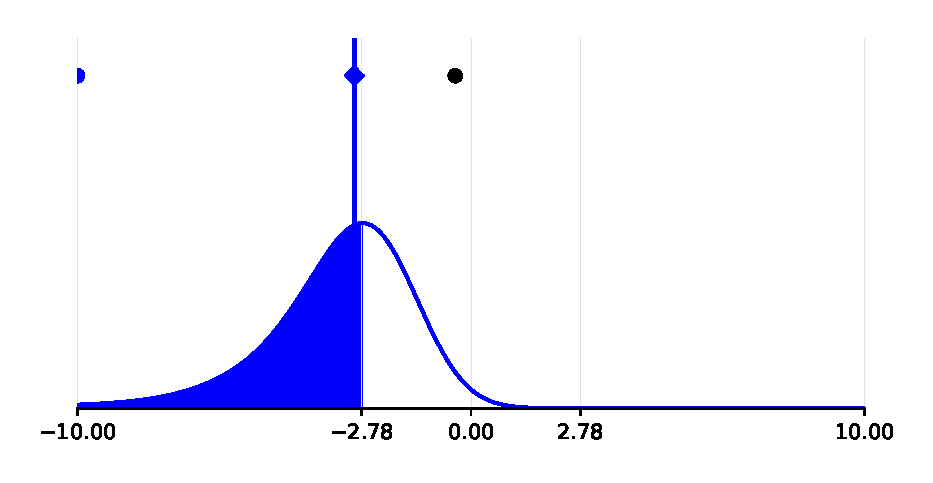
\includegraphics[width=7.5cm, trim=30 0 30 0]{figures/sonar_0.eps}}\\

\midrule	&\textsc{gnb} & \textsc{knn} & \textsc{t} & p & \textsc{i} & \textsc{d}\\
	\color{blue} $\approx$ & \color{blue}  0.683 &\color{blue}  \bfseries 0.805 & -2.96 & 0.04 & --- & ---\\\midrule
	{\bfseries\color{black}\tiny=}& \color{black} \bfseries 0.695 & \color{black} \bfseries 0.719 & -0.40 & 0.71 & 3354 & \color{black} 0.4383\\
	{\bfseries\color{blue}\tiny-}& \color{blue}  0.666 & \color{blue} \bfseries 0.811 & -106.50 & 0.00 & 4661 & \color{blue} 0.5617\\
	{\tiny+}& --- & --- & --- & --- & --- & ---\\
\bottomrule
\end{tabular}
}
\end{table}

The table header contains the name of a data set for which the experiment was carried out (in this case \textsc{sonar}), and directly below it the T-statistics distribution in the population of ten thousand experiments, in the form of gaussian estimation, in the range from -10 to 10. Additional vertical lines represents the point 0 and the significance limits for the adopted $\alpha$ (0.05) and the division method used, with four points of freedom (approximately 2.78).

%W nagłówku tabeli znajduje się zbiór danych, dla którego przeprowadzono eksperyment (w tym przypadku sonar), a bezpośrednio pod nim wykres rozkładu T-statystyki w populacji dziesięciu tysięcy eksperymentów, w postaci estymacji gaussa, w przedziale od -10 do 10. Dodatkowymi pionowymi liniami zaznaczono punkt 0 oraz granice istotności dla przyjętego alpha = .05 oraz, wynikających z zastosowanej metody podziału, czterech punktów swobody (w przybliżeniu 2.78).

The chart is supplemented with four additional sets of values in the following rows of the table:

%Wykres uzupełniany jest o cztery dodatkowe zbiory wartości w kolejnych rzędach tabeli:

\begin{itemize}
	\item $\approx$ : the average value of the sample from ten thousand courses.
	\item $=$ : the value of the sample with the T-statistic nearest to zero, contained in the statistical non-significant interval, symbolizing the lack of significant differences between the compared algorithms
	\item $-$ : the value of the observation with the lowest T-statistic outside the statistical non-significant interval, symbolizing a statistically significant advantage of the algorithm from the right column,
	\item $+$ : the value of the observation with the highest T-statistic outside the statistical non-significant interval, symbolizing a statistically significant advantage of the algorithm from the left column.
\end{itemize}

The next columns in the table are mean accuracies obtained by compared algorithms, T-statistics (column T), p-value (p), seed value which allowed to obtain a given division-observation (\textsc{i}) and the percentage of observations in which the situation described in the line occurred (\textsc{d}).

%Kolejne kolumny w tabeli to porównywane algorytmy, T-statystyka (kolumna T), p-wartość (p), wartość ziarna, która pozwoliła na uzyskanie zadanego podziału-obserwacji (I) oraz odsetek obserwacji, w których zaszła opisywana w wierszu sytuacja (D).

Therefore, the interpretation of the example table will be as follows. The average value of the observation indicates the predominance of the KNN algorithm over GNB, for the former the accuracy of approximately 81\%, and for the second 68\%. The average T-statistics value is -2.96, which gives p-value at 0.04, which makes it a statistically significant difference.

%W związku z tym, interpretacja przykładowej tabeli będzie następująca. Uśredniona wartość obserwacji wskazuje na przewagę algorytmu KNN nad GNB, dla tego pierwszego przyjmując dokładność około 81\%, a dla drugiego 68\%. Uśredniona wartość T-statystyki wynosi -2.96, co daje p-wartość na poziomie 0.04, a więc jest to różnica istotna statystycznie.

However, we may also observe situations in which a significant difference between algorithms does not occur (line $=$). An example is the partition instance obtained for random seed 3354, where T-statistic equal -0.4, which gives p-value at 0.71. Similar situations (no significant difference) occurs in 44\% of the considered cases. Divisions which show a significant advantage of the KNN algorithm occur in 56\% of cases, and the extreme value of T-statistics is -106.5, which is an outlier in the context of the problem under consideration.

%Możemy jednak zaobserwować też sytuacje, w których istotna różnica pomiędzy algorytmami nie występuje (wiersz $=$). Przykładem jest instancja podziału uzyskana dla ziarna 3354, gdzie T-statystyka wynosi -0.4, co daje p-wartość na poziomie 0.71. Podobne sytuacje (braku istotnej różnicy) występują w 44\% rozpatrywanych przypadków. Podziały, które wykazują istotną przewagę algorytmu KNN występują w 56\% przypadków, a skrajną wartością T-statystyki jest -106.5, co stanowi obserwację odstającą w kontekście rozpatrywanego problemu.

In connection with the above observations, we can properly validate two contradictory research hypotheses by pulling the dataset into folds adequately many times. Moreover, with the average value of T-statistics close to the significance threshold, approximately half of the experiments will give us information about the KNN advantage, when the other half of the divisions will deny any statistical difference.

%W związku z powyższymi obserwacjami, odpowiednio wiele razy losując podział zbioru danych na foldy, możemy należycie uprawdopodobnić dwie sprzeczne ze sobą hipotezy badawcze. Co więcej, przy średniej wartości T-statystyki bliskiej progowi istotności, w przybliżeniu około połowa eksperymentów da nam informację o przewadze KNN, kiedy druga połowa podziałów jej zaprzeczy.

The simplest of situations encountered in performed experiments is that in which each of ten thousand experiments leads to the same conclusion, as is shown in the examples in the Table \ref{tab:single}. The distribution of T-statistics in such cases is either narrow enough to fit within the statistical irrelevance interval (\textsc{soybean}) or far enough from it, so that even outlier observations leading to other conclusions do not happen. It is worth noting, however, that even in such cases, outliers reveal a major deviation from the mean value (for example, an average of 10.56 in the \textsc{wine} dataset and an outlier observation of 114.79). It is particularly important to note at this point that only six of the fifty-four comparisons are characterized by such unambiguous conclusions.

%Najprostszą z sytuacji napotkanych w zrealizowanych eksperymentach jest ta, w której każdy z dziesięciu tysięcy eksperymentów prowadzi do tego samego wniosku, jak przedstawiono to na przykładach w Tabeli \ref{tab:single}. Rozkład T-statystyki w takich przypadkach jest albo na tyle wąski, aby zmieścić się w przedziale nieistotności statystycznej (zbiór soybean) albo na tyle odległy od niego, aby nie zdarzały się nawet obserwacje odstające prowadzące do innych wniosków. Warto jednak zauważyć, że nawet w takich przypadkach obserwacje odstające wykazują pokaźne odchylenie od normy (przykładowo średnie 10.56 w zbiorze wine i obserwacja odstająca o wartości 114.79). Szczególnie istotnym jest zauważenie w tym punkcie, że jedynie sześć z pięćdziesięciu czterech porównań charakteryzuje się takimi, jednoznacznymi wnioskami.
%(JEDEN --- 6 PRZYKŁADÓW na 54)


\begin{table}[!h]
	\centering
	\caption{Example}
	\label{tab:single}
	\resizebox{.323\textwidth}{!}{%
\begin{tabular}{c||cc||c|c|c||c}
	\toprule
	\multicolumn{7}{c}{\textsc{wine}}\\
	\bottomrule
	\multicolumn{7}{c}{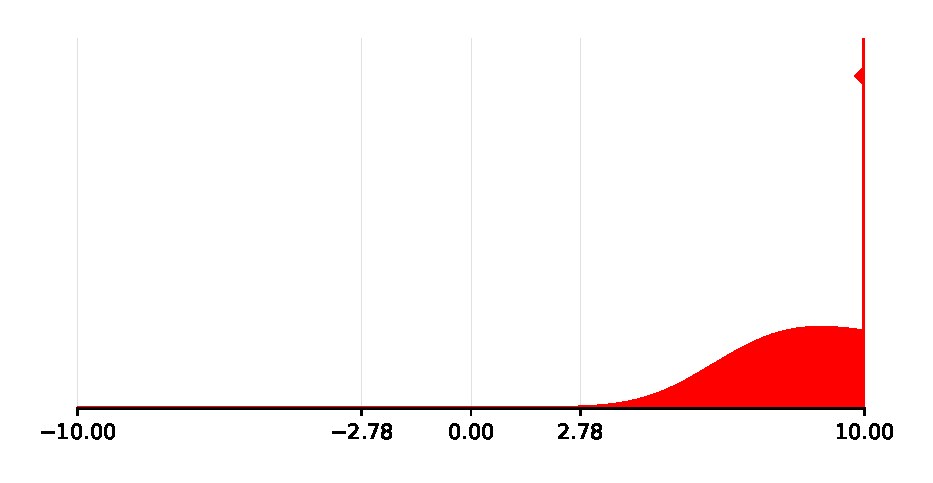
\includegraphics[width=7.5cm, trim=30 0 30 0]{figures/wine_0.eps}}\\

\midrule	&\textsc{gnb} & \textsc{knn} & \textsc{t} & p & \textsc{i} & \textsc{d}\\
	\color{red} $\approx$ & \color{red} \bfseries 0.972 &\color{red}   0.703 & 10.56 & 0.00 & --- & ---\\\midrule
	{\tiny=}& --- & --- & --- & --- & --- & ---\\
	{\tiny-}& --- & --- & --- & --- & --- & ---\\
	{\bfseries\color{red}\tiny+}& \color{red} \bfseries 0.976 & \color{red}  0.677 & 114.79 & 0.00 & 744 & \color{red} 1.0000\\
	\bottomrule
\end{tabular}
}\resizebox{.31\textwidth}{!}{%
\begin{tabular}{c||cc||c|c|c||c}
	\toprule
	\multicolumn{7}{c}{\textsc{soybean}}\\
	\bottomrule
	\multicolumn{7}{c}{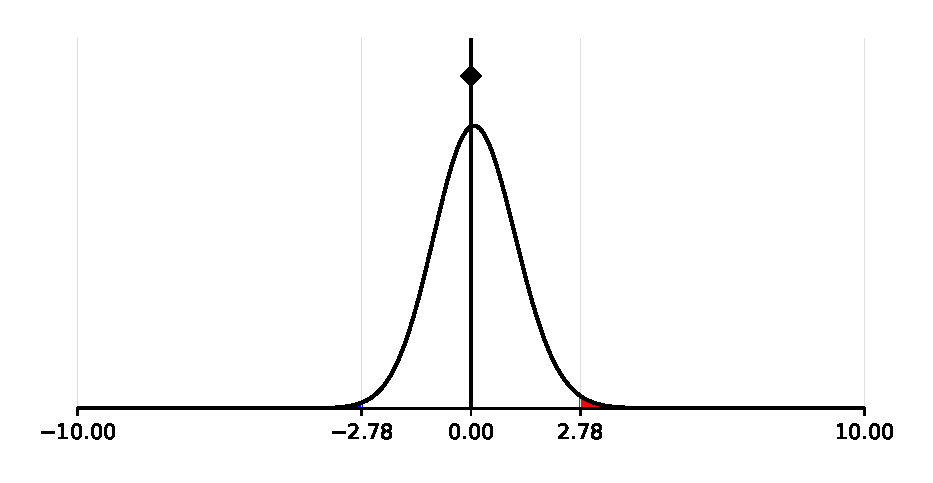
\includegraphics[width=7.5cm, trim=30 0 30 0]{figures/soybean_1.eps}}\\

\midrule	&\textsc{gnb} & \textsc{dtc} & \textsc{t} & p & \textsc{i} & \textsc{d}\\
	\color{black} $\approx$ & \color{black} \bfseries 1.000 &\color{black}  \bfseries 1.000 & 0.00 & 1.00 & --- & ---\\\midrule
	{\bfseries\color{black}\tiny=}& \color{black} \bfseries 1.000 & \color{black} \bfseries 1.000 & 0.00 & 1.00 & 0 & \color{black} 1.0000\\
	{\tiny-}& --- & --- & --- & --- & --- & ---\\
	{\tiny+}& --- & --- & --- & --- & --- & ---\\
	\bottomrule
\end{tabular}
}\resizebox{.334\textwidth}{!}{%
\begin{tabular}{c||cc||c|c|c||c}
	\toprule
	\multicolumn{7}{c}{\textsc{monkone}}\\
	\bottomrule
	\multicolumn{7}{c}{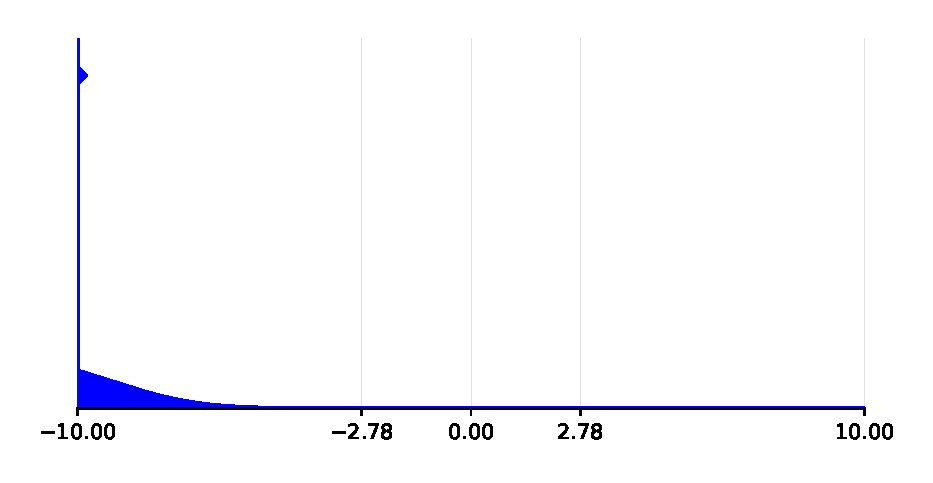
\includegraphics[width=7.5cm, trim=30 0 30 0]{figures/monkone_0.eps}}\\

\midrule	&\textsc{gnb} & \textsc{knn} & \textsc{t} & p & \textsc{i} & \textsc{d}\\
	\color{blue} $\approx$ & \color{blue}  0.664 &\color{blue}  \bfseries 0.946 & -15.84 & 0.00 & --- & ---\\\midrule
	{\tiny=}& --- & --- & --- & --- & --- & ---\\
	{\bfseries\color{blue}\tiny-}& \color{blue}  0.667 & \color{blue} \bfseries 0.946 & -248.20 & 0.00 & 3069 & \color{blue} 1.0000\\
	{\tiny+}& --- & --- & --- & --- & --- & ---\\
\bottomrule\end{tabular}
}
\end{table}

The dominant majority, as many as 39 out of 54 comparisons correspond to the situation presented in the example in Table 1, where we can draw two contradictory conclusions from the appropriate (let's emphasize - random) combination of patterns division into folds. Examples here are presented in Table \ref{tab:double}. In the case of the \textsc{wine} dataset, we may observe a situation in which the GNB algorithm in averaging achieves an advantage over the DTC, but in as many as three out of ten cases, random division of the data set will lead to the conclusion that there are no significant differences. A much more interesting case is the \textsc{iris} dataset, where in 99\% of divisions there is no significant difference between the compared classifiers, but 1\% of the problem instances leads to the conclusion that the KNN has a significant advantage over GNB. An even stronger example of this type is the \textsc{australian} dataset, where, despite the predominance of the DTC over the KNN and the average difference in quality at 13\%, we can still find two parts-per-thousand of situations in which the difference between them disappears.

%Dominująca większość, bo aż 39 z 53 porównań odpowiada sytuacji przedstawionej w przykładzie z Tabeli 1, gdzie możemy wyciągnąć dwa sprzeczne wnioski z odpowiedniej (podkreślmy -- losowej) kombinacji wzorców w podziale na foldy. Przykłady tutaj prezentuje Tabela \ref{tab:double}. W wypadku zbioru wine widzimy sytuację, w której algorytm GNB w uśrednieniu osiąga przewagę nad DTC, ale w aż trzech na dziesięć przypadków, losowy podział zbioru danych doprowadzi do wniosku o braku istotnych różnic. Znacznie ciekawszy jest przypadek zbioru iris, gdzie w 99\% podziałów nie ma istotnej różnicy pomiędzy porównywanymi klasyfikatorami, ale 1\% instancji problemu prowadzi do wniosku o istotnej przewadze KNN. Jeszcze silniejszym przykładem tego rodzaju jest zbiór australian, gdzie mimo dominacji wniosku o istotnej przewadze DTC nad KNN i średniej różnicy w ich jakości na poziomie 13 \%, nadal możemy odnaleźć dwa promile sytuacji, w których istotność różnicy między nimi zanika.


%(DWA --- 39 PRZYKŁADÓW)


\begin{table}[!h]
	\centering
	\caption{Example}
	\label{tab:double}
	\resizebox{.321\textwidth}{!}{%
\begin{tabular}{c||cc||c|c|c||c}
	\toprule
	\multicolumn{7}{c}{\textsc{wine}}\\
	\bottomrule
		\multicolumn{7}{c}{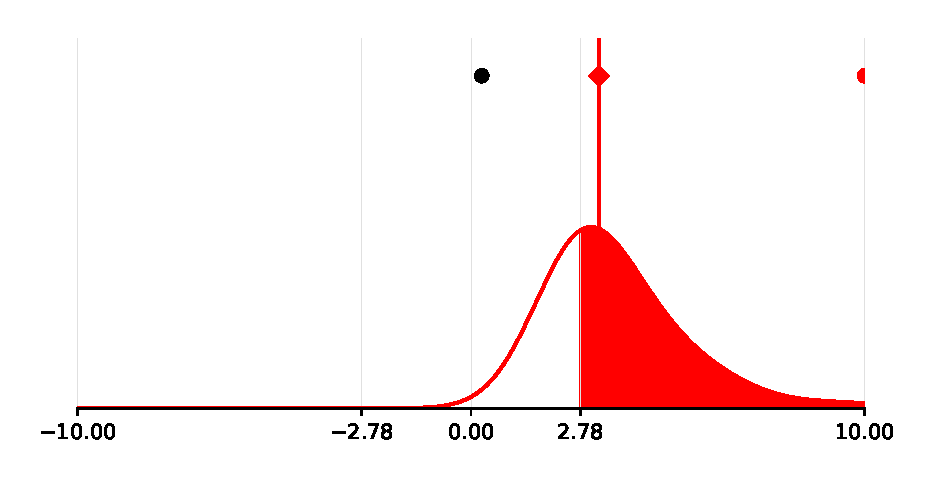
\includegraphics[width=7.5cm, trim=30 0 30 0]{figures/wine_1.eps}}\\

\midrule	&\textsc{gnb} & \textsc{dtc} & \textsc{t} & p & \textsc{i} & \textsc{d}\\
	\color{red} $\approx$ & \color{red} \bfseries 0.972 &\color{red}   0.917 & 3.25 & 0.03 & --- & ---\\\midrule
	{\bfseries\color{black}\tiny=}& \color{black} \bfseries 0.972 & \color{black} \bfseries 0.966 & 0.27 & 0.80 & 650 & \color{black} 0.3246\\
	{\tiny-}& --- & --- & --- & --- & --- & ---\\
	{\bfseries\color{red}\tiny+}& \color{red} \bfseries 0.971 & \color{red}  0.886 & 58.74 & 0.00 & 6516 & \color{red} 0.6754\\
	\bottomrule
\end{tabular}
}\resizebox{.325\textwidth}{!}{%
\begin{tabular}{c||cc||c|c|c||c}
	\toprule
	\multicolumn{7}{c}{\textsc{iris}}\\
	\bottomrule
	\multicolumn{7}{c}{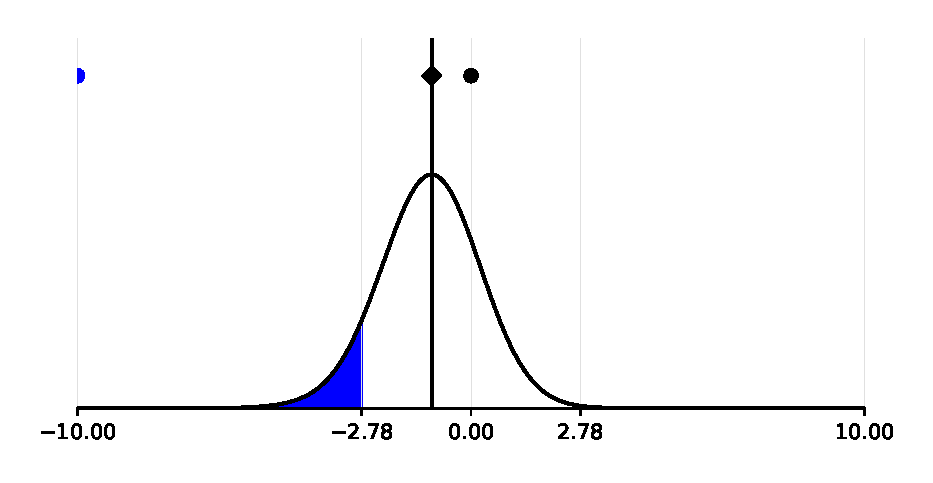
\includegraphics[width=7.5cm, trim=30 0 30 0]{figures/iris_0.eps}}\\

\midrule	&\textsc{gnb} & \textsc{knn} & \textsc{t} & p & \textsc{i} & \textsc{d}\\
	\color{black} $\approx$ & \color{black} \bfseries 0.967 &\color{black}  \bfseries 0.967 & -1.00 & 0.37 & --- & ---\\\midrule
	{\bfseries\color{black}\tiny=}& \color{black} \bfseries 0.960 & \color{black} \bfseries 0.960 & 0.00 & 1.00 & 0 & \color{black} 0.9872\\
	{\bfseries\color{blue}\tiny-}& \color{blue}  0.946 & \color{blue} \bfseries 0.980 & -146.00 & 0.00 & 213 & \color{blue} 0.0128\\
	{\tiny+}& --- & --- & --- & --- & --- & ---\\
	\bottomrule
\end{tabular}
}\resizebox{.325\textwidth}{!}{%
\begin{tabular}{c||cc||c|c|c||c}
	\toprule
	\multicolumn{7}{c}{\textsc{australian}}\\
	\bottomrule
	\multicolumn{7}{c}{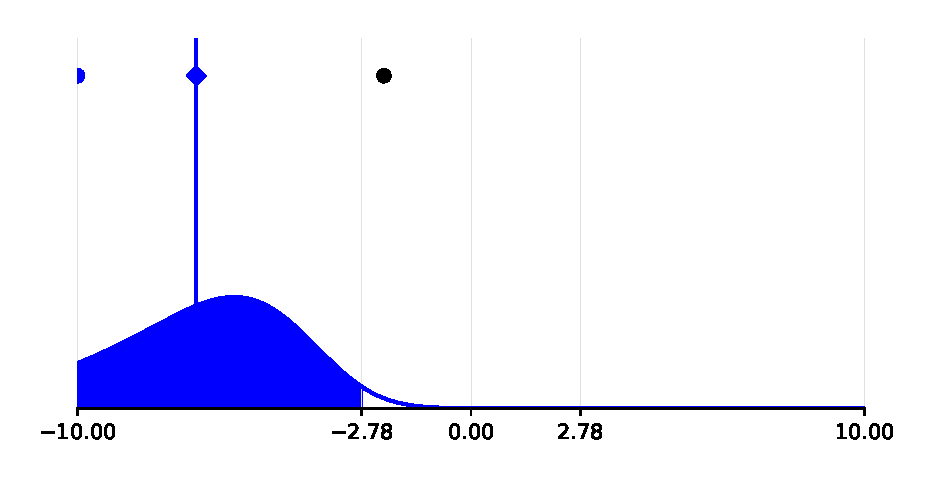
\includegraphics[width=7.5cm, trim=30 0 30 0]{figures/australian_2.eps}}\\

\midrule	&\textsc{knn} & \textsc{dtc} & \textsc{t} & p & \textsc{i} & \textsc{d}\\
	\color{blue} $\approx$ & \color{blue}  0.693 &\color{blue}  \bfseries 0.820 & -6.98 & 0.00 & --- & ---\\\midrule
	{\bfseries\color{black}\tiny=}& \color{black} \bfseries 0.679 & \color{black} \bfseries 0.774 & -2.21 & 0.09 & 6575 & \color{black} 0.0021\\
	{\bfseries\color{blue}\tiny-}& \color{blue}  0.694 & \color{blue} \bfseries 0.839 & -72.59 & 0.00 & 3782 & \color{blue} 0.9979\\
	{\tiny+}& --- & --- & --- & --- & --- & ---\\
\bottomrule\end{tabular}
}
\end{table}

The most interesting, however, is the third, last group of observations, which consists of 9 out of 54 examples (Table \ref{tab:triple}). There is a set of cases in which, depending on which of the random dataset divisions we select for the experiment, we can get the validation of each possible conclusion. The liver dataset is particularly interesting here, where only eight out of ten thousand cases show the DTC algorithm superiority over KNN, with approximately 90\% of their equal quality and 10\% of KNN advantage cases.

This may lead to the hypothesis that if we have sufficiently large computational power to repeat random dataset divisions, we will lead to a situation in which, using the standard approach to experiments, we will be able to reasonably substantiate any hypothesis about the statistical relationship between the compared classifiers. Moreover, on the basis of all separate groups of cases, we can certainly conclude that the existence of such combinations of data sets and classification algorithms is common, against which we can substantiate contradictory hypotheses, depending on the applied random division of the data set into folds.


\begin{table}[!h]
	\centering
	\caption{Example}
	\label{tab:triple}
	\resizebox{.328\textwidth}{!}{%
\begin{tabular}{c||cc||c|c|c||c}
	\toprule
	\multicolumn{7}{c}{\textsc{liver}}\\
	\bottomrule
		\multicolumn{7}{c}{\includegraphics[width=7.5cm, trim=30 0 30 0]{figures/liver_2.eps}}\\
\midrule	&\textsc{knn} & \textsc{dtc} & \textsc{t} & p & \textsc{i} & \textsc{d}\\
	\color{black} $\approx$ & \color{black} \bfseries 0.667 &\color{black}  \bfseries 0.638 & 1.18 & 0.29 & --- & ---\\\midrule
	{\bfseries\color{black}\tiny=}& \color{black} \bfseries 0.637 & \color{black} \bfseries 0.637 & 0.00 & 1.00 & 722 & \color{black} 0.8828\\
	{\bfseries\color{blue}\tiny-}& \color{blue}  0.663 & \color{blue} \bfseries 0.689 & -8.96 & 0.00 & 8873 & \color{blue} 0.0008\\
	{\bfseries\color{red}\tiny+}& \color{red} \bfseries 0.669 & \color{red}  0.611 & 341.00 & 0.00 & 4553 & \color{red} 0.1164\\
\bottomrule
\end{tabular}
}\resizebox{.321\textwidth}{!}{%
\begin{tabular}{c||cc||c|c|c||c}
	\toprule
	\multicolumn{7}{c}{\textsc{german}}\\
	\bottomrule
	\multicolumn{7}{c}{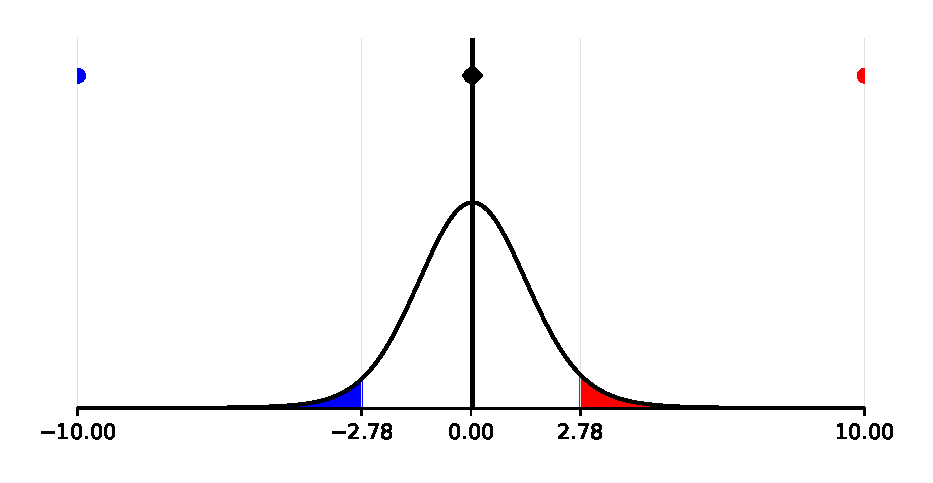
\includegraphics[width=7.5cm, trim=30 0 30 0]{figures/german_2.eps}}\\
\midrule	&\textsc{knn} & \textsc{dtc} & \textsc{t} & p & \textsc{i} & \textsc{d}\\
	\color{black} $\approx$ & \color{black} \bfseries 0.690 &\color{black}  \bfseries 0.690 & 0.04 & 0.55 & --- & ---\\\midrule
	{\bfseries\color{black}\tiny=}& \color{black} \bfseries 0.678 & \color{black} \bfseries 0.678 & 0.00 & 1.00 & 1082 & \color{black} 0.9686\\
	{\bfseries\color{blue}\tiny-}& \color{blue}  0.681 & \color{blue} \bfseries 0.710 & -9.98 & 0.00 & 9310 & \color{blue} 0.0136\\
	{\bfseries\color{red}\tiny+}& \color{red} \bfseries 0.695 & \color{red}  0.662 & 12.92 & 0.00 & 4886 & \color{red} 0.0178\\
\bottomrule
\end{tabular}
}\resizebox{.325\textwidth}{!}{%
\begin{tabular}{c||cc||c|c|c||c}
	\toprule
	\multicolumn{7}{c}{\textsc{diabetes}}\\
	\bottomrule
	\multicolumn{7}{c}{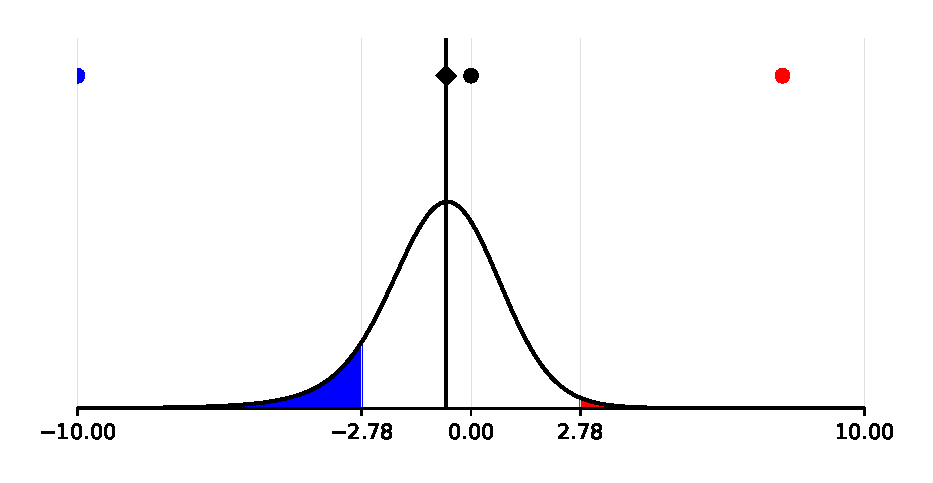
\includegraphics[width=7.5cm, trim=30 0 30 0]{figures/diabetes_2.eps}}\\

\midrule	&\textsc{knn} & \textsc{dtc} & \textsc{t} & p & \textsc{i} & \textsc{d}\\
	\color{black} $\approx$ & \color{black} \bfseries 0.688 &\color{black}  \bfseries 0.699 & -0.63 & 0.47 & --- & ---\\\midrule
	{\bfseries\color{black}\tiny=}& \color{black} \bfseries 0.687 & \color{black} \bfseries 0.687 & 0.00 & 1.00 & 3549 & \color{black} 0.9441\\
	{\bfseries\color{blue}\tiny-}& \color{blue}  0.681 & \color{blue} \bfseries 0.733 & -14.88 & 0.00 & 8407 & \color{blue} 0.0529\\
	{\bfseries\color{red}\tiny+}& \color{red} \bfseries 0.708 & \color{red}  0.674 & 7.92 & 0.00 & 9658 & \color{red} 0.0030\\
\bottomrule\end{tabular}
}
\end{table}

\end{document}
